\chapter{Preliminary Concepts}\label{chp:preliminary-concepts}

In this chapter, we introduce the fundamental concepts necessary for
understanding this thesis. In this work, we employ basic concepts from
Combinatorial Optimization, which are assumed to be known. If the reader deems a
review necessary, we recommend the textbook by Nemhauser and
Wolsey~\cite{Nemhauser}, which covers this topic with a focus on \gls{ilp}, one
of the main tools used in this work. Basic concepts related to graph theory are
also assumed to be known. Should the reader require a refresher, the material
can be found in standard textbooks on the subject, such as
Diestel~\cite{diestel:2005}.

\section{Integer Linear Programming}\label{sec:integer-linear-programming}
A \gls{lp} problem consists of maximizing (or minimizing) a linear objective function subject to a set of linear constraints. An \gls{lp} can be formulated as
\begin{equation}
	\text{(PLP)}:\quad \max \{ c x : A x \; f \; b, \; x \in \mathbb{R}^n \},
\end{equation}
where $A$ is an $m \times n$ real matrix, $b$ and $c$ are real vectors of dimensions $m \times 1$ and $1 \times n$, respectively, and $x$ is a vector of $n$ decision variables.
The set of all $x \in \mathbb{R}^n$ satisfying the constraints defines the feasible region of the \gls{lp}. Because all inequalities are linear, this region forms a convex polyhedron, and if it is bounded, the optimal solution of the \gls{lp} lies at one of its vertices.

\gls{lp} problems can be solved in polynomial time using algorithms such as the ellipsoid method or interior-point methods (see Chapters 8 and 9 of Bertsimas and Tsitsiklis~\cite{bertsimas1997introduction}). Despite its exponential worst-case complexity, the simplex method often performs efficiently in practice and remains the most widely used approach.

When the decision variables $x$ are restricted to take integer values, the problem becomes an \gls{ilp} problem, which can be expressed as
\begin{equation}
	\text{(PILP)}:\quad \max \{ c x : A x \; f \; b, \; x \in \mathbb{Z}^n \}.
\end{equation}
Although \gls{lp}s can be solved in polynomial time, \gls{ilp}s are generally NP-hard, and many combinatorial optimization problems can be modeled in this way.

By relaxing the integrality constraints of PILP, one obtains the linear relaxation of the \gls{ilp}. Let $Q \subset \mathbb{R}^n$ denote the feasible region satisfying $A x \; f \; b$, and let $P = Q \cap \mathbb{Z}^n$ denote the set of feasible integer solutions. The polyhedron $Q$ is said to be a formulation (or model) of the \gls{ilp}. Among the infinitely many possible formulations satisfying $P = Q \cap \mathbb{Z}^n$, one of particular theoretical interest is the convex hull of $P$, denoted $\text{CH}(P)$---the smallest convex polyhedron containing all integer feasible points.

Ideally, one would have $\text{CH}(P) = Q$, as solving the linear relaxation would then yield the exact \gls{ilp} optimum in polynomial time. However, for NP-hard problems, the convex hull is typically defined by an exponential number of inequalities, making it computationally intractable.

In practice, the solution process usually begins by solving the linear relaxation of PILP. If the resulting optimal solution is integral, it is also optimal for the \gls{ilp}. Otherwise, additional methods such as cutting planes and branch-and-bound are employed. Cutting plane methods iteratively refine the formulation by adding valid inequalities to better approximate $\text{CH}(P)$, whereas branch-and-bound algorithms recursively partition the problem into smaller subproblems. The combination of both strategies results in the branch-and-cut algorithm, discussed next.

\subsection{Cutting Planes and Polyhedral Combinatorics}

Consider again the (PILP) problem and the polyhedra $Q$ and $\text{CH}(P)$ defined above. Suppose the linear relaxation $Q$ is solved to optimality, yielding an optimal fractional solution $x^* \in Q \setminus \text{CH}(P)$.

An inequality is said to be valid for a polyhedron $D$ if all points in $D$ satisfy it. A cutting plane (or simply cut) is a valid inequality for $\text{CH}(P)$ that is violated by $x^*$. The purpose of a cutting plane algorithm is to find such inequalities and iteratively add them to the formulation $Q$, thereby tightening it (i.e., reducing $Q \setminus \text{CH}(P)$).

The search for a valid inequality violated by a given fractional point constitutes the separation problem, and the method used to identify such inequalities is known as the separation method. After each cut is added, the linear relaxation is re-solved. This process repeats until the optimal solution of the relaxation becomes integral.

There are infinitely many possible cuts that can separate a fractional point $x^*$ from $\text{CH}(P)$, and the effectiveness of the algorithm depends strongly on the choice of cuts. Cuts that more closely approximate $\text{CH}(P)$ generally yield faster convergence. The intersection between a cutting plane and $\text{CH}(P)$ defines a face of $\text{CH}(P)$. Faces of $\text{CH}(P)$ of dimension $\dim(\text{CH}(P)) - 1$ are called facets, and characterizing facet-defining inequalities is a central objective in the study of polyhedral combinatorics.

\subsection{Branch-and-Bound and Branch-and-Cut}\label{sec:branch-and-bound-and-branch-and-cut}

The \gls{bb} algorithm is a refinement of exhaustive search that systematically decomposes the solution space $X$ of a combinatorial optimization problem into smaller subsets $X_1, X_2, \ldots, X_k$, such that
\begin{equation}
	X = \bigcup_{i=1}^{k} X_i.
\end{equation}
This decomposition process, known as branching, recursively subdivides the feasible region into smaller subproblems, each defined over a subset $X_i \cap S$, where $S \subseteq X$ denotes the feasible set. The solutions of these subproblems collectively contain the global optimum.

The resulting hierarchy of subproblems can be represented as a search tree, where each node corresponds to a subproblem and its children to further subdivisions. Initially, the tree contains only the root node, representing the original problem. As branching proceeds, additional nodes are generated.

To avoid enumerating all possible nodes, the algorithm maintains bounds on the objective value of each subproblem: a dual bound $z_i$ (upper bound for maximization problems) and a primal bound $\bar{z}_i$ (lower bound from feasible solutions). The best feasible solution found so far is called the incumbent, with value $z^*$. A node is pruned, i.e., not further decomposed, under one of the following conditions:
\begin{enumerate}
	\item \textbf{Optimality:} $z_i = \bar{z}_i$;
	\item \textbf{Infeasibility:} the subproblem has no feasible solutions;
	\item \textbf{Bounding:} $z_i < z^*$, meaning the node cannot yield a better solution than the incumbent.
\end{enumerate}
The algorithm terminates when no active nodes (i.e., unprocessed nodes) remain in the tree.

When applied to ILP, the process begins by solving the linear relaxation at the root node. If the resulting solution $x^*$ is integral, it is optimal for the ILP. Otherwise, a fractional variable $x_i^*$ is selected for branching, creating two new subproblems with additional constraints $x_i \le \lfloor x_i^* \rfloor$ and $x_i \ge \lceil x_i^* \rceil$. The selection of the branching variable significantly affects performance, making branching strategies a critical aspect of effective ILP solution methods.

A \gls{bc} algorithm integrates cutting plane procedures within the branch-and-bound framework. Typically, cutting planes are applied at each node before branching, according to predefined stopping criteria, such as limits on computation time, the number of iterations, or the number of cuts added.

Branch-and-cut algorithms are particularly effective for ILPs whose formulations contain an exponential number of constraints. In such cases, only a subset of inequalities is included initially, with additional constraints generated on demand through the separation method as violations are detected during the search. When the separation problem can be solved in polynomial time, only a polynomially bounded number of constraints needs to be generated, due to the established equivalence between the optimization and separation problems for a given polyhedron~\cite{groetschel1988geometric}. Further details on linear and integer programming can be found in~\cite{bertsimas1997introduction, wolsey1998integer}.

\section{Lagrangean Relaxation}\label{sec:cbrp-lagrangean-relaxation}

\gls{lr} is a well-known decomposition method used to solve combinatorial
optimization problems. The main idea of \gls{lr} is to remove complicated
constraints from the mathematical model and transfer them to the objective
function by assigning them weights (known as Lagrange multipliers), which
penalize their violation in any solution. It can be shown that the cost of an
optimal solution to the \gls{lr} always provides a dual bound for the optimal
value of the original problem. A primal bound can be obtained by checking the
feasibility of a solution returned by the relaxed model and computing the value
of the original objective function for that solution. An important step in
\gls{lr} is determining the values of the Lagrange multipliers that yield the
best dual bound. For this purpose, the subgradient method can be employed, which
is an iterative procedure in which the multipliers are updated until they
converge to their optimal values. For a minimization problem, this method can be
interpreted as the maximization of the lower bound obtained from the relaxed
model based on appropriate choices of multipliers~\cite{Beasley:1993}.

\gls{lr} is particularly convenient for problems that, apart from a subset of
complicating constraints, can be efficiently solved. For instance, consider the
following \gls{ilp} model:

\begin{align*}
	\text{(IP) } &              &  & z = \min cx           &  &  &  &  &  &  &  & \\
	             & \text{s.t. } &  & Ax \geq b,            &  &  &  &  &  &  &  & \\
	             &              &  & Dx \geq d,            &  &  &  &  &  &  &  & \\
	             &              &  & x \in \mathbb{Z}^n_+. &  &  &  &  &  &  &  &
\end{align*}

Assuming $Dx \geq d$ is the set of complicating constraints, removing it yields
$z' = \min \{cx : x \in X\}$, where $X = \{x \in \mathbb{Z}^n_+ : Ax \geq b\}$,
which is an easier problem and referred to as the relaxed problem. Two facts can
be observed. First, $z'$ is a lower (dual) bound on $z$, since the feasible
region of $x$ is larger, so the optimal value of $z'$ is less than or equal to
that of $z$. Second, the optimal solution in $X$ may not satisfy the constraints
in $Dx \geq d$. Based on these observations, the idea is to move the
complicating constraints into the objective function, penalizing their violation
using a vector $u \in \mathbb{R}^{m}_+$. This results in the Lagrangian
relaxation problem (\gls{lpp}), which can be written as:

\begin{align*}
	\text{LR($u$) } &              &  & z(u) = \min cx + u(d - Dx) &  &  &  &  &  &  & \\
	                & \text{s.t. } &  & x \in X,                   &  &  &  &  &  &  & \\
	                &              &  & u \in \mathbb{R}^m_+.      &  &  &  &  &  &  &
\end{align*}

The following proposition establishes the relationship between $z(u)$ and $z$.

\begin{proposition}
	Let $z(u) = \min \{cx + u (d - Dx) : x \in X\}$. Then, $z(u) \leq z$ for all $u \geq 0$.
\end{proposition}

The penalty $u_i$ associated with constraint $D_ix \geq d_i$ is called the
Lagrange multiplier for that constraint. We now define the following problem:
determine the set of multipliers that provide the best (i.e., greatest) dual
bound $z(u)$. To find these values, we must solve the Lagrangian dual problem
(\gls{ldp}), described as:

\begin{align*}
	\text{LD } &  &  & w = \max \{z(u) : u \geq 0\}. &  &  &  &  &
\end{align*}

The Lagrangian dual can be solved using the subgradient optimization method,
which is based on the following result.

\begin{proposition} \label{proposition:convex}
	A function $g : \mathbb{R}^n \rightarrow \mathbb{R}$ is concave if and only if, for every $\bar{x} \in \mathbb{R}^n$, there exists $s \in \mathbb{R}^n$ such that $g(\bar{x}) + s(x - \bar{x}) \geq g(x)$ for all $x \in \mathbb{R}^n$.
\end{proposition}

Thus, at point $\bar{x}$, it is necessary to choose a direction in which to move
to increase $g(x)$. From Proposition~\ref{proposition:convex}, we know that if
$g(x) > g(\bar{x})$, then $s(x - \bar{x}) > 0$. That is, moving an appropriate
amount in the direction of $s$ from $\bar{x}$ will increase the value of $g$.
Therefore, we must find a vector $s$ that satisfies
Proposition~\ref{proposition:convex}. When $g$ is differentiable at $\bar{x}$,
we can take $s = \nabla g(\bar{x})$, i.e., the gradient of $g$ at $\bar{x}$.
However, when $g$ is not differentiable, Proposition~\ref{proposition:convex}
still guarantees the existence of a vector $s$ such that $s(x^* - \bar{x}) > 0$
for an optimal point $x^*$. This means it is possible to move from $\bar{x}$ a
small step in the direction of $s$ to get closer to an optimal point, even if
$g$ does not increase. Before finding such a vector $s$, we define the notions
of subgradient and subdifferential.

\begin{definition}\label{definition:subgradient}
	Let $g : \mathbb{R}^n \rightarrow \mathbb{R}$ be a concave function. A vector $s$ is a subgradient of $g$ at $\bar{x}$ if and only if $s(x - \bar{x}) \geq g(x) - g(\bar{x})$ for all $x \in \mathbb{R}^n$. The subdifferential $(\delta g(\bar{x}))$ of $g$ at $\bar{x}$ is the set of all subgradients at that point.
\end{definition}

An immediate consequence of the above is the following:

\begin{proposition}\label{proposition:optimal}
	If $g$ is concave and $0 \in \delta g(x^*)$, then $g(x^*) = \max\{g(x) : x \in \mathbb{R}^n\}$, that is, $x^*$ is an optimal solution.
\end{proposition}

Therefore, in theory, to maximize a concave function $g$, it is sufficient to
start from any point and iteratively take small steps in the direction of a
subgradient at that point until $0$ belongs to the subdifferential of the
current point—that is, the current point is optimal. The results below allow us
to apply this theory to the Lagrangian relaxation technique for \gls{ilp}.

\begin{proposition} \label{proposition-zu-convex}
	$z(u) = \min \{cx + u (d - Dx)\}$ is concave.
\end{proposition}

The next result shows how to compute a subgradient of $z(u) = \min \{cx + u (d -
	Dx) : x \in X\}$ at point $u$.

\begin{proposition}
	Let $\bar{x} \in X$ such that $z(u) = c \bar{x} + u(d - D\bar{x})$. Then, $(d - D\bar{x})$ is a subgradient of $z(u)$ at $u$.
\end{proposition}

Based on the previous definitions and results, we can now present a procedure to
minimize a concave function for which a subgradient is known at all points in
its domain. For this purpose, a high-level pseudocode of the subgradient method
is presented in Algorithm~\ref{code:subgradient}.

\begin{algorithm}[!ht]
	\caption{\label{code:subgradient} Subgradient Method (Minimization Problem)}
	\SetAlgoLined
	\KwData{threshold, maxIter, updatePi}
	\KwResult{$z_{LB}$, $z_{UB}$}
	$m \leftarrow \rho \leftarrow 0$\;
	$z_{LB} \leftarrow 0$\;
	$z_{UB} \leftarrow$ cost of a feasible solution\;
	$\alpha^{0} \leftarrow \theta^{0} \leftarrow 0$\; $\pi^{0} \leftarrow 2$\;

	\While{$(\frac{z_{UB} - z_{LB}}{Z_{UB}}) \leq \ threshold$  or $m \ < \ maxIter$}{
		$x \leftarrow$ solution of $LR(\alpha^{m})$\;
		$z^{m} \leftarrow$ cost of the objective function of $x$ \;
		\If{$z^{m} > z_{LB}$}{
			$z_{LB} \leftarrow z^{m}$\;
		}
		$z_f^m \leftarrow$ original objective function value of solution $x$\;
		\uIf{$x$ is feasible and $z_f^m < z_{UB}$}{
			$z_{UB} \leftarrow z_f^m$\;
			$\rho \leftarrow 0$\;
		} \Else {
			$\rho \leftarrow \rho + 1$\;
		}

		\If{$\rho \ = \ updatePi$}{
			$\pi \leftarrow \pi/2$\;
			$\rho \leftarrow 0$\;
		}

		$\theta^{m} \leftarrow$ subgradient($x$)\;
		$n^{m} \leftarrow $ norm($\theta^{m}$)\;
		$s^{m} \leftarrow \pi^{m} \frac{(z_{UB} - z^{m})}{(n^{m})^{2}}$\;

		$\alpha^{m+1} \leftarrow \max(0, \alpha^{m} + s^{m}\theta^{m})$\;

		$m \leftarrow m + 1$\;
	}
\end{algorithm}

The algorithm takes three input parameters: `threshold', `maxIter', and
`updatePi'. The first two are stopping criteria. The `threshold' indicates the
maximum gap value for the solution to be considered optimal, terminating the
execution. The `maxIter' limits the maximum number of iterations of the
subgradient method. The third parameter, `updatePi`, is a counter for updating
the value of $\pi$, i.e., when `updatePi` consecutive iterations occur without
improvement in the dual bound. Lines (1)–(5) represent the initialization of
variables: $m$ is the main loop counter, and $\rho$ counts consecutive
iterations without improvement in $z_{UB}$. The variables $z_{LB}$ and $z_{UB}$
are the lower and upper bounds, respectively.

The symbol $\alpha$ represents the vector of Lagrange multipliers, and $\theta$
is the subgradient vector. First, the Lagrangian primal problem is solved using
the current multipliers, and this solution is used to obtain the subgradient. If
the relaxed model returns a better feasible solution (lower in value), $z_{UB}$
is updated; if the solution is feasible for the original problem, $z_{LB}$ is
updated with the value of the original objective function, disregarding the cost
of the multipliers. The subgradient vector ($\theta^m$) is then calculated, and
its norm ($n^m$) is used to compute the step size ($s^m$) in the subgradient
direction. The Lagrange multipliers are then updated for the next iteration.
Line (26) ensures non-negativity of the multipliers.

\section{Optimization Under Uncertainty}\label{sec:optimization-under-uncertainty}

This Section presents the basic concepts of Stochastic Programming and is
strongly based on the textbook by Birge and Louveaux~\cite{birge:2011}.

Two-Stage Stochastic Programming models with recourse deal with uncertain data,
represented by random variables. A decision must be made at the present time; we
call this the first-stage (or first-phase) decision, and at a later time, after
its implementation, the uncertainties are revealed. Then, based on the
first-stage decision and the revealed uncertain data, we can make a corrective
(recourse) decision, called the second-stage (or second-phase)
decision~\cite{birge:2011}.

The uncertain data of the problem are represented by a random vector~$\xi$. We
are interested in the case where~$\xi$ is a discrete random variable, that is,
it can take values from a finite set $\Xi = \{\xi_{1}, \ldots, \xi_{k}\}$. We
denote each possible random event by $\omega \in \Omega$. Alternatively, $\xi$
can be represented as a function of $\omega \in \Omega$, with $\xi(\omega)$
being the value taken by the random variable when event $\omega$ occurs.

First-stage decision variables are represented by vector~$x$, of
dimension~$n_{1}$, while second-stage decision variables are represented by the
random vector~$y$, of dimension~$n_{2}$. We denote by $y(\omega)$ the
second-stage decision variables associated with the realization of random
event~$\omega$.

A traditional two-stage stochastic programming problem, also called a \gls{rp}
or \emph{here-and-now} problem, since a decision must be made in the present
before the uncertainties are revealed, is formulated as:
\begin{align}
	\max \quad        & c^{T} x + \mathbb{E}_{\xi} \left[ \max q(\omega)^{T} y(\omega) \right] \nonumber \\
	\text{s.t.} \quad & A x = b \nonumber                                                                \\
	                  & T(\omega)x + W y(\omega) = h(\omega) \nonumber                                   \\
	                  & x \geq 0 \nonumber                                                               \\
	                  & y(\omega) \geq 0
	\label{eq:rp}
\end{align}

The first-stage data matrices and vectors $A$, $b$, and $c$ have dimensions
$m_{1} \times n_{1}$, $m_{1}$, and $n_{1}$, respectively. Once uncertainties are
revealed through the realization of event $\omega \in \Omega$, $T(\omega)$,
$h(\omega)$, and $q(\omega)$, with dimensions $m_{2} \times n_{1}$, $m_{2}$, and
$n_{2}$, respectively, become known. To represent the problem's uncertainties as
a single random vector, we define
\[
	\xi(\omega)^{T} = \left(q(\omega)^{T}, \; h(\omega)^{T}, \; T_{1\cdot}(\omega), \ldots, T_{m_{2}\cdot}(\omega) \right),
\]
for every $\omega \in \Omega$, where $T_{i\cdot}(\omega)$ denotes the $i$-th row
of matrix $T(\omega)$. We are interested in the class of \emph{fixed recourse
	problems}~\cite{birge:2011}, in which the matrix $W$, of dimension $m_{2}
	\times n_{2}$, represents the second-stage actions and does not depend on the
realization of the random event, and is thus known before making the first-stage
decision.

Note that the objective function in~\eqref{eq:rp} has a deterministic term
$c^{T}x$ and the expected value of $q(\omega)^{T} y(\omega)$ over all
realizations~$\omega$. What makes solving a two-stage stochastic program
difficult is that, for each $\omega \in \Omega$, determining $y(\omega)$
requires solving a \gls{lp} (or \gls{ilp}) problem. To make this more explicit,
an alternative notation for the same problem is known as the \emph{deterministic
	equivalent program}. For a given realization~$\omega$ and first-stage
decision~$x$, we define:
\[
	Q(x, \xi(\omega)) = \max_{y} \left\{ q(\omega)^{T} y \; \middle| \; W y = h(\omega) - T(\omega) x, \; y \geq 0 \right\},
\]
as the second-stage value function. Then, the expected second-stage value for
the first-stage decision~$x$ is:
\[
	Q(x) = \mathbb{E}_{\xi} \left[ Q(x, \xi) \right].
\]
With this, the deterministic equivalent program can be formulated as:
\begin{align}
	\max \quad        & c^{T} x + Q(x) \nonumber \\
	\text{s.t.} \quad & A x = b \nonumber        \\
	                  & x \geq 0.
	\label{eq:rp_det}
\end{align}

\subsection{Expected Value of Perfect Information (EVPI)}

The \gls{evpi} measures the maximum amount a decision-maker would be willing to
pay to have perfect foresight of the future. This allows determining to what
extent a more accurate forecast would improve the quality of the obtained
solution. Consider:
\begin{align}
	\max \quad        & z(x, \xi(\omega)) = c^{T} x + Q(x, \xi(\omega)) \nonumber \\
	\text{s.t.} \quad & A x = b \nonumber                                         \\
	                  & x \geq 0,
	\label{eq:scenario_problem}
\end{align}
which is the optimization problem for a given scenario $\xi(\omega)$. We assume
that for every $\xi(\omega) \in \Xi$, this problem is neither infeasible nor
unbounded.

Suppose there is an efficient way to obtain an optimal solution
$\bar{x}(\xi(\omega))$ to~\eqref{eq:scenario_problem} for
scenario~$\xi(\omega)$, and let $z(\bar{x}(\xi(\omega)), \xi(\omega))$ be its
objective value. The so-called \emph{wait-and-see} (WS) solution is given by:

\begin{equation}
	WS = \mathbb{E}_{\xi} \left[ z(\bar{x}(\xi), \xi) \right].
	\label{eq:ws}
\end{equation}

That is, for each scenario $\xi(\omega)$, we solve~\eqref{eq:scenario_problem}
to optimality and take the expected value of the objective over all $\omega \in
	\Omega$. The \gls{rp}, defined by~\eqref{eq:rp} or~\eqref{eq:rp_det}, can be
written as:

\begin{equation}
	RP = \max_{x} \mathbb{E}_{\xi} \left[ z(x, \xi) \right].
	\label{eq:rp_exp}
\end{equation}
By definition, the \gls{evpi} is the difference between the wait-and-see and
here-and-now solutions:
\[
	EVPI = WS - RP.
\]

\subsection{Value of the Stochastic Solution}

A practical difficulty of the wait-and-see approach is that we must solve a
subproblem for each scenario~$\xi(\omega)$. A simpler approach is to replace the
random vector~$\xi$ with its expected value $\bar{\xi} = \mathbb{E}[\xi]$. This
problem is known as the \gls{evp}, or \emph{mean value
	problem}~\cite{birge:2011}. This corresponds to a simpler problem than the
recourse problem, since we only solve for a single future scenario. The
objective of the \gls{evp} is:

\begin{equation}
	EV = \max z(x, \bar{\xi}).
	\label{eq:evp}
\end{equation}

Let $\bar{x}(\bar{\xi})$ be an optimal solution to~\eqref{eq:evp}. Given the
stochastic nature of the problem, in general $\bar{x}(\bar{\xi})$ may not be
close to the optimal solution of the recourse problem~\eqref{eq:rp}. However,
this solution is useful for defining the \gls{vss}, which measures the quality
of the solution in terms of~\eqref{eq:rp}. We define the expected value of the
\gls{evp} solution as:

\begin{equation}
	EEV = \mathbb{E}_{\xi} \left[ z(\bar{x}(\bar{\xi}), \xi) \right].
	\label{eq:eev}
\end{equation}

This is equivalent to solving the recourse problem while fixing the first-stage
decision obtained from the \gls{evp}. Given the EEV, the \gls{vss} is:
\[
	VSS = RP - EEV,
\]
which indicates the loss incurred by adopting only the expected scenario
$\bar{\xi}$ compared to the full recourse problem~\eqref{eq:rp}. This
corresponds to the cost of ignoring uncertainty. The values $WS$~\eqref{eq:ws},
$RP$~\eqref{eq:rp_exp}, and $EEV$~\eqref{eq:eev} satisfy:
\[
	EEV \leq RP \leq WS.
\]
Thus, for a maximization problem, EEV  and wait-and-see serve, respectively, as
lower and upper bounds for the problem of interest, the recourse problem.

\section{Stochastic Optimization Models}\label{sec:cbrp-stochastic-models}

The stochastic version of the \gls{cbrp}, called in this work as \gls{scbrp},
computes, in the first-stage, a route to nebulize the blocks in the scenario $0$
(present), in which the objective is to maximize the profit considering a bonus
related to the impact on the reduction of future cases for each scenario in the
second-stage. The second-stage represents a set of independent routes that
nebulize independent blocks in each future scenario.

In addition to the deterministic data, a set of $k$ future scenarios $\Omega =
	\{\omega_1, \dots, \omega_k\}$, with $\xi^{\omega}$ being the probability of
scenario $\omega \in \Omega$ to occur. The profit of block $b$ in the
present is $p_{b}^{0}$, and the profit in each future scenario is
$p_{b}^{\omega}$. This value represents the number of cases predicted for
that city block in the scenario $\omega$. However, the profit of each block
is affected by the first-stage, with a parameter $\alpha$ being a reduction
factor in the number of cases in a block nebulized in the first-stage. For
example, if $\alpha = 1$, then for all block $\{b \in B: y_{b}^{0} = 1\}$
will have a $0$ profit in all second-stage scenarios.

Let $\Omega' = \{0, \omega_1, \dots, \omega_k\}$ be the augmented set of
scenarios, with $0$ representing the present scenario and $\omega_1, \dots,
	\omega_k$ representing the $k$ future scenarios. The following binary decision
variables are introduced for the \gls{scbrp} model:

\begin{itemize}
	\item $y_{b}^{\omega} \in \{0, 1\}$: binary variable valued as 1 if the block $b \in B$ is nebulized in the scenario $\omega \in \Omega'$ ($y_{b}^{\omega} = 1$) or not ($y_{b}^{\omega} = 0$).
	\item $x_{a}^{\omega} \in \{0, 1\}$: binary variable valued as 1 if the arc $a \in A'$ is used in the route in the scenario $\omega \in \Omega'$ ($x_{a}^{\omega} = 1$) or not ($x_{a}^{\omega} = 0$).
	\item $z_{b}^{\omega} \in \mathbb{R}$: real variable that represents the maximum profit of a block $b \in B$ in a scenario $\omega \in \Omega'$ ($z_{b}^{\omega} \in \mathbb{R}_{+}$).
\end{itemize}

The \gls{scbrp} formulation is defined as follows:

\begin{align}
	\text{(Path-SCBRP)} & \max \overbrace{\sum_{b \in B} y_{b}^{0}(p_{b}^{0} + \alpha \sum_{\omega \in \Omega} \xi^{\omega} p_{b}^{\omega})}^{\text{First-Stage}} + \overbrace{\sum_{\omega \in \Omega} \xi^{\omega} \sum_{b \in B} z_{b}^{\omega}}^{\text{Second-Stage}} & \label{eq:sof}
\end{align}
\begin{align}
	\nonumber \text{subject to:} &                                                                                                         &                                                                                     \\
	                             & z_{b}^{\omega} \leq y_{b}^{\omega}((1 - \alpha)p_{b}^{\omega}) + (1 - y_{b}^{0})(\alpha p_{b}^{\omega}) & \forall b \in B, \omega \in \Omega \label{eq:stochastic-z-value}                    \\
	                             & z_{b}^{\omega} \leq y_{b}^{\omega}p_{b}^{\omega}                                                        & \forall b \in B, \omega \in \Omega \label{eq:stochastic-z-y-value}                  \\
	                             & \sum_{i \in V} x_{0,i}^{\omega} = \sum_{j \in V} x_{j,0}^{\omega} = 1                                   & \forall \omega \in \Omega' \label{eq:stochastic-s-t-all}                            \\
	                             & \sum_{i \in V} x_{i,j}^{\omega} - \sum_{k \in V} x_{j,k}^{\omega} = 0                                   & \forall j \in V, \omega \in \Omega' \label{eq:stochastic-flow-conservation}         \\
	                             & \sum_{j \in \delta^{-}(i)} x_{i,j}^{\omega} \geq y_{b}^{\omega}                                         & \forall b \in B, i \in V(b), \omega \in \Omega' \label{eq:stochastic-in-path}       \\
	                             & \sum_{(i, j) \in A} x_{i,j}^{\omega}t_{i,j} + \sum_{b \in B} y_{b}^{\omega}t^{'}_{b} \leq T             & \forall \omega \in \Omega' \label{eq:stochastic-max-time}                           \\
	                             & \sum_{(i, j) \in A(C)} x_{i,j}^{\omega} \leq |V(C)| - 1                                                 & \forall C \subseteq V, \omega \in \Omega' \label{eq:stochastic-subtour-elimination} \\
	                             & x \in \mathbb{B}^{|A'| * |\Omega'|}                                                                     & \label{eq:stochastic-dom-x}                                                         \\
	                             & y \in \mathbb{B}^{|B| * |\Omega'|}                                                                      & \label{eq:stochastic-dom-y}                                                         \\
	                             & z \in \mathbb{R}_{+}^{|B| * |\Omega|}                                                                   & \label{eq:stochastic-dom-z}
\end{align}

The objective function~\eqref{eq:sof} maximizes the total profit. When a block
is attended in the first-stage, the final value is the profit of the block in
scenario $0$ plus $\alpha$ times the profit for all scenarios multiplied by the
probability of the scenario $\omega$ to occur. Besides the profit associated in
first-stage, the second-stage maximizes the profit for the residual number of
cases (after the $\alpha$ reduction for apply the route in scenario $0$) in each
block and for every future scenario $\omega \in \Omega$.

Constraints~\eqref{eq:stochastic-z-value} ensure that the profit of a block $b$
in the scenario $\omega$ is $(1 - \alpha) p_{b}^{\omega}$, if $y_{b}^{0} = 1$ or
$p_{b}^{\omega}$ when $y_{b}^{0} = 0$.
Constraints~\eqref{eq:stochastic-z-y-value}  guarantee that the value of
$z_{b}^{\omega}$ is $0$ when $y_{b}^{\omega} = 0$ and $p_{b}^{\omega}$
otherwise. The Constraints from~\eqref{eq:stochastic-s-t-all}
to~\eqref{eq:stochastic-subtour-elimination} are the same as the constraints
from~\eqref{eq:s-t-all} to~\eqref{eq:circuit-subtour-elimination} of the
Path-CBRP formulation, but for independent routes for all scenario $\omega \in
	\Omega'$. Constraints~\eqref{eq:stochastic-dom-x}-\eqref{eq:stochastic-dom-z}
define the domain of the decision variables.

Considering the Path-SCBRP formulation, with the changes to consider the
stochastic nature of the problem, it is also possible to adapt the deterministic
models from Section~\ref{sec:cbrp-deterministic-models} to generate feasible
solutions for the \gls{scbrp}, i.e., creating the $k$ routes to nebulize the
blocks in the scenario $0$ and each future scenario. The further references for
the \gls{scbrp} will follow the same pattern presented for the deterministic
formulations: Path-SCBRP, Path-SCBRP-MTZ, Walk-SCBRP and Walk-SCBRP-MTZ.

\section{Multi-Agent-Based Simulation}\label{sec:multi-agent-simulation}

Epidemiological models aim to answer how a certain disease spreads in a region
and how it may appear in regions not initially considered susceptible. Since
simulation models have limitations regarding the real world, they commonly
attempt to represent a phenomenon either at a global (macro) or local (micro)
scale.

Macro-simulation is a deterministic approach that focuses on representation at a
global level, neglecting individual characteristics such as sex, age, address,
and interactions between individuals. Although easy to interpret and implement,
when using a macro model, one must be aware of these limitations since certain
individual characteristics may be crucial to disease
propagation~\citep{damien:2017}. On the other hand, micro-simulation models
contain a particular representation for each individual.

Multi-agent systems commonly represent complex systems with characteristics such
as non-linearity and multiple levels of abstraction~\citep{furtado:2015}. This
system contains agents that perceive and act on the environment, reacting to
situations and making decisions based on cognitive abilities. Typically,
predicting the global behavior of \gls{mabs} is impractical because individual
interactions between agents lead to emergent global structures.

\gls{mabs} encompass various types tailored to simulate complex systems where
multiple autonomous entities interact dynamically. One prevalent type is
task-based \gls{mabs}, focusing on agents completing specific tasks or goals
within a system. These simulations are crucial in studying decentralized systems
like logistics and manufacturing.

Furthermore, spatial \gls{mabs} integrates geographic information and spatial
relationships, essential for modeling urban planning, environmental systems, and
epidemiology. Adaptive \gls{mabs} introduces agents capable of learning and
adapting behaviors over time, necessary for studying adaptive systems such as
artificial intelligence and robotics. Lastly, hybrid \gls{mabs} combines
features from multiple types, offering versatility to model various real-world
phenomena across domains like economics, biology, and engineering. Each kind of
\gls{mabs} contributes uniquely to understanding complex systems and addressing
challenges in predictive modeling and policy analysis~\citep{Bonabeau:2002}.

Due to the inherent non-deterministic nature of \gls{mabs}, multiple simulation
runs are required to achieve statistically significant results and accurately
characterize system behavior. The complex interactions between input parameters
and output behaviors in MABS often make it challenging to establish explicit
relationships and formally validate models. To overcome this, researchers
frequently employ expert validation, as seen
in~\cite{amouroux:2008,damien:2017}, where epidemiological experts were
consulted to evaluate the model's realism and reliability.

Regardless of the scale, it is possible to use compartmental theory, where the
main idea is to represent the states of individuals~\citep{brauer-2008}. In our
Dengue spread simulation, we adopted the following states: susceptible (S),
exposed or latent (E), infected (I), and recovered (R) as illustrated in
Figure~\ref{fig:dynamicmodel}. Individuals who have never been exposed to the
disease are in state S. If an individual carries the virus but does not yet
transmit it or show symptoms, they are in state E. Symptoms appear when they
reach state I, which also allows the individual to transmit the infection. In
the R state, individuals are considered cured and immune to new infections.

\begin{figure}[!ht]
	\centering

	\resizebox{0.75\columnwidth}{!}{
		\tikzset{every picture/.style={line width=0.75pt}} %set default line width to

	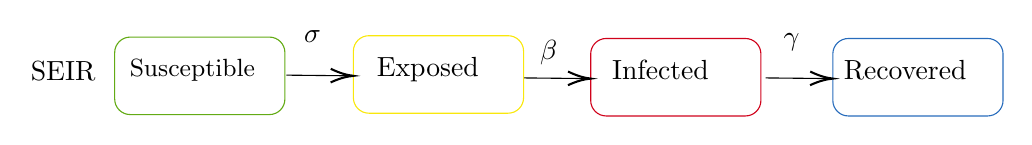
\begin{tikzpicture}[x=0.75pt,y=0.75pt,yscale=-1,xscale=1]
		%uncomment if require: \path (0,300); %set diagram left start at 0, and has
		%height of 300

		%Rounded Rect [id:dp9217887491174969] 
		\draw  [color={rgb, 255:red, 99; green, 171; blue, 21 }  ,draw opacity=1 ]
		(62.33,41.47) .. controls (62.33,37.34) and (65.68,34) .. (69.8,34) --
		(136.87,34) .. controls (140.99,34) and (144.33,37.34) .. (144.33,41.47) --
		(144.33,63.87) .. controls (144.33,67.99) and (140.99,71.33) .. (136.87,71.33)
		-- (69.8,71.33) .. controls (65.68,71.33) and (62.33,67.99) .. (62.33,63.87) --
		cycle ;
		%Rounded Rect [id:dp36097559929859013] 
		\draw  [color={rgb, 255:red, 208; green, 2; blue, 27 }  ,draw opacity=1 ]
		(291.67,42.13) .. controls (291.67,38.01) and (295.01,34.67) .. (299.13,34.67)
		-- (366.2,34.67) .. controls (370.32,34.67) and (373.67,38.01) .. (373.67,42.13)
		-- (373.67,64.53) .. controls (373.67,68.66) and (370.32,72) .. (366.2,72) --
		(299.13,72) .. controls (295.01,72) and (291.67,68.66) .. (291.67,64.53) --
		cycle ;
		%Straight Lines [id:da9742211892376831] 
		\draw    (259.33,53.67) -- (289.67,53.98) ; \draw [shift={(291.67,54)}, rotate =
			180.59] [color={rgb, 255:red, 0; green, 0; blue, 0 }  ][line width=0.75]
		(10.93,-3.29) .. controls (6.95,-1.4) and (3.31,-0.3) .. (0,0) .. controls
		(3.31,0.3) and (6.95,1.4) .. (10.93,3.29)   ;
		%Rounded Rect [id:dp37752716490425275] 
		\draw  [color={rgb, 255:red, 40; green, 108; blue, 188 }  ,draw opacity=1 ]
		(408.33,42.13) .. controls (408.33,38.01) and (411.68,34.67) .. (415.8,34.67) --
		(482.87,34.67) .. controls (486.99,34.67) and (490.33,38.01) .. (490.33,42.13)
		-- (490.33,64.53) .. controls (490.33,68.66) and (486.99,72) .. (482.87,72) --
		(415.8,72) .. controls (411.68,72) and (408.33,68.66) .. (408.33,64.53) -- cycle
		;
		%Straight Lines [id:da2512507786148114] 
		\draw    (376,53.67) -- (406.33,53.98) ; \draw [shift={(408.33,54)}, rotate =
			180.59] [color={rgb, 255:red, 0; green, 0; blue, 0 }  ][line width=0.75]
		(10.93,-3.29) .. controls (6.95,-1.4) and (3.31,-0.3) .. (0,0) .. controls
		(3.31,0.3) and (6.95,1.4) .. (10.93,3.29)   ;
		%Rounded Rect [id:dp4832950812851634] 
		\draw  [color={rgb, 255:red, 249; green, 231; blue, 9 }  ,draw opacity=0.99 ]
		(177.33,40.8) .. controls (177.33,36.68) and (180.68,33.33) .. (184.8,33.33) --
		(251.87,33.33) .. controls (255.99,33.33) and (259.33,36.68) .. (259.33,40.8) --
		(259.33,63.2) .. controls (259.33,67.32) and (255.99,70.67) .. (251.87,70.67) --
		(184.8,70.67) .. controls (180.68,70.67) and (177.33,67.32) .. (177.33,63.2) --
		cycle ;
		%Straight Lines [id:da02397316252168946] 
		\draw    (145,52.33) -- (175.33,52.65) ; \draw [shift={(177.33,52.67)}, rotate =
			180.59] [color={rgb, 255:red, 0; green, 0; blue, 0 }  ][line width=0.75]
		(10.93,-3.29) .. controls (6.95,-1.4) and (3.31,-0.3) .. (0,0) .. controls
		(3.31,0.3) and (6.95,1.4) .. (10.93,3.29)   ;


		% Text Node
		\draw (68.33,43.33) node [anchor=north west][inner sep=0.75pt]   [align=left]
		{{\small Susceptible}};
		% Text Node
		\draw (300.67,44) node [anchor=north west][inner sep=0.75pt]   [align=left]
		{Infected};
		% Text Node
		\draw (412.33,44) node [anchor=north west][inner sep=0.75pt]   [align=left]
		{Recovered};
		% Text Node
		\draw (266,34.07) node [anchor=north west][inner sep=0.75pt]    {$\beta $};
		% Text Node
		\draw (383.33,31.07) node [anchor=north west][inner sep=0.75pt]    {$\gamma $};
		% Text Node
		\draw (187.33,42.67) node [anchor=north west][inner sep=0.75pt]   [align=left]
		{Exposed};
		% Text Node
		\draw (152.33,29.73) node [anchor=north west][inner sep=0.75pt]    {$\sigma $};
		% Text Node
		\draw (20.67,44.33) node [anchor=north west][inner sep=0.75pt]   [align=left]
		{SEIR};


	\end{tikzpicture}

	} \caption{Diagram of a dynamic compartmental model.}
	\label{fig:dynamicmodel}
\end{figure}

The compartment flow is based on the order of the letters~\citep{amaku:2014}.
For example, an SEIR model states that individuals are initially susceptible to
the virus or disease, then they become exposed, infected, and finally recover.
The transition between states is not mandatory and depends on the model's
internal parameters, which aim to be as coherent as possible with reality. The
choice of a model depends primarily on the intrinsic characteristics of the
disease. The literature has proposed a set of different models considering
various types of compartments, such as \textbf{SEI}~\cite{Scoglio2021,
	Puntipa2023}, \textbf{SEIR}~\cite{Scoglio2021, Puntipa2023, Meng2023,
	da-silva:2020}, and \textbf{SIR}~\cite{Umar2022, Prasetyo2023, Srivastav2023},
among others.  Classical mathematical models are mainly based on compartmental
theory, and a system of \gls{ode} describes the changes between
states~\citep{da-silva:2020}.

\section{Simheuristics}\label{sec:simheuristics}

Simulation methods are widely used to analyze complex real-life systems under
uncertainty, which is typically modeled through probability
distributions~\cite{lucas:2015}. These techniques are applied in diverse domains
such as manufacturing, logistics, transportation, healthcare, finance, smart
cities, and telecommunications. While simulation provides valuable insights into
system performance under different scenarios, it does not inherently offer
optimization capabilities, especially for large-scale and NP-hard
\gls{scop}~\cite{juan:2022}. To address this, simulation is often combined with
metaheuristics, which can efficiently explore large solution spaces and deliver
high-quality solutions in reasonable computational times.

The hybridization of simulation and optimization, known as
simulation-optimization, encompasses various methods including mathematical
programming, metaheuristics, and machine learning. In such approaches,
simulation can serve multiple roles: evaluating objective functions or
constraints in stochastic settings, generating feasible solutions, or enhancing
analytical models~\cite{juan:2015}. Surrogate models derived from simulation
outputs can further accelerate the optimization process. This integration
enables a balance between modeling realism and computational tractability,
making simulation-optimization a first-choice strategy for tackling complex
stochastic problems~\cite{juan:2022}.

Given a deterministic optimization problem, it is reasonable to assume that its
optimal and near-optimal solutions will exhibit satisfactory performance when
moderate levels of uncertainty are introduced~\cite{juan:2022}. Formally, for a
solution $s$, let $\text{det}(s)$ denote its deterministic performance and
$\text{stoch}(s)$ its stochastic performance (estimated via simulation). Under
moderate uncertainty, these values are expected to be strongly and positively
correlated. However, this correlation diminishes as uncertainty increases, and
for large variances, robust or reliable solutions may be preferable to those
merely maximizing expected performance.

Another important observation concerns the use of the best deterministic
solution $\text{det}(s^*)$. In many optimization problems, the optimal objective
value degrades as uncertainty increases, particularly when asymmetric effects
are present, where detrimental realizations of random variables outweigh
beneficial ones. Let $s^*$ denote an optimal or near-optimal deterministic
solution, and $s^{**}$ an optimal or near-optimal stochastic solution. Then, for
minimization problems, it often holds that $\text{det}(s^*) \leq
	\text{stoch}(s^{**}) \leq \text{stoch}(s^*)$, while for maximization problems,
$\text{stoch}(s^*) \leq \text{stoch}(s^{**}) \leq \text{det}(s^*)$. Thus,
deterministic optimal values provide natural lower and upper bounds for their
stochastic counterparts~\cite{juan:2022}.

\Cref{fig:logic-simheuristics} shows the default logic behind simheuristic
concept. Given a stochastic optimization problem, its deterministic counterpart
is considered. This can be done, for instance, by replacing all random variables
by their expected values, which leads to a simplified version of the stochastic
problem in which uncertainty is not considered. Then, a metaheuristic component
is employed to efficiently search inside the solution space, thus generating
increasingly better solutions to the deterministic version of the problem. Each
time the metaheuristic generates a ``promising'' solution (i.e., one that is
likely to perform well in a scenario under uncertainty), this solution is sent
to the simulation component in order to assess its performance in the stochastic
environment.

The simulation component returns not only estimates of statistics, such as the
mean, variance, and percentiles associated with the proposed solution, but also
probabilistic information that can be useful in risk or reliability analyses, as
well as information about the status of different system variables. Since
simulation is a time consuming procedure, it is usually a good idea to employ a
short number of simulation runs every time a new promising solution is evaluated
at this stage, otherwise the simulation computing time might jeopardize the time
required by the metaheuristic to converge to near-optimal solutions.  Some
useful recommendations to speed up these computations can be found in
Rabe~\cite{rabe:2020}.

The feedback provided by the simulation can then be processed by a machine
learning component and then used to: (i) update and adjust the metaheuristic
parameters to better explore the solution space and increase the chances of
obtaining new solutions with a high stochastic performance; (ii) build a
classification or prediction model able to identify new promising solutions with
a high accuracy, thus avoiding wasting time in simulating solutions that will
offer sub-optimal values under uncertainty conditions; and (iii) develop a
surrogate model that, at least partially, substitutes time-consuming simulations
when estimating the value of the stochastic objective function or probabilistic
constraints associated with a new promising solution proposed by the
metaheuristic component

As a result of this first stage, a reduced list of ``elite'' solutions is
obtained. According to our initial estimates, each of these solutions show a
high performance in a scenario under uncertainty. Now, in order to increase the
accuracy of our estimates, a more intensive simulation is executed on each of
the elite solutions. Of course, variance reduction techniques, such as the use
of common random numbers, can be employed here to speed up these simulations,
which can also be run in parallel processors. As a final stage, the simulation
outcomes might be employed to perform a risk or reliability analysis on each of
these elite solutions. This analysis might enrich the decision-making process
with detailed probabilistic information describing the stochastic behavior of
each elite solution.

\begin{figure}[h!]
	\centering
	\begin{tikzpicture}
		[
			node distance=1.9cm, % distance between nodes
			font=\tiny,
			align=center
		]

		% Defining styles
		\tikzstyle{startstop} = [rectangle, rounded corners, minimum width=3cm, minimum height=1cm, text centered, draw=black, text width=3cm, fill=blue!30!white]

		%%%%%%%%%%%%%%%%%%%%%%%%%%%%%%%%%%%%%%%%%%%%%%%%%%%%%%%%%%%%%%%%%%%%%%%

		\tikzstyle{io} = [ellipse, minimum width=2cm, text width=2cm, minimum height=1cm, text centered, draw=black, fill=gray!30!white, font=\bf\tiny]

		\tikzstyle{process} = [tape, minimum width=1.5cm, text width=2cm, minimum height=1cm, text centered, draw=black, fill=green!30!white, font=\bf\tiny]

		\tikzstyle{decision} = [diamond, text width=1.5cm, aspect=2, text height=1, text centered, draw=black, fill=yellow!30!white, font=\bf\tiny]

		\tikzstyle{stage} = [rectangle, minimum width=1cm, text width=1cm, minimum height=1cm, draw=black, font=\bf\tiny]

		\tikzstyle{artificial} = [rectangle, draw=white, font=\bf\tiny]

		\tikzstyle{arrow} = [thick,->,>=stealth]

		% Create states
		\node (start) [startstop] at (0, 0) {Stochastic\\Optimization\\Problem};

		\node (deterministic) [startstop, right of=start, xshift=7cm] {Deterministic\\Optimization\\Problem};

		% Links
		\draw [arrow] (start) -- node[text width=3cm, fill=white, align=center] {Replacement of Random Elements} (deterministic);

		%%%%%%%%%%%%%%%%%%%%%%%%%%%%%%% Stage 1 %%%%%%%%%%%%%%%%%%%%%%%%%%%%%%
		%%%%%%%%%%%%%%%%%%%%%%%%%%%%%%%%%%%%%%%%%%%%%%%%%%%%%%%%%%%%%%%%%%%%%%
		\node (metaheuristic) [process, below of=deterministic] {Metaheuristic Algorithm};

		\node (deterministic-sol) [io, below of=metaheuristic] {New Deterministic Solution};
		\node (ml-component) [process, below of=deterministic-sol] {Machine Learning Component};
		\node (fast-sim-component) [process, below of=ml-component] {Fast Simulation Component};

		\node (promissing-sol) [decision, xshift=-2.5cm, left of=ml-component] {Promissing\\Solution?};
		\node (surrogate-sol) [decision, xshift=-2.5cm, left of=fast-sim-component] {Surrogate\\Model\\Available?};

		\node (surrogate-component) [process, below of=surrogate-sol] {Surrogate Model};

		\node (update-sol-list) [io, below of=surrogate-component] {Update Solution List};

		\node (available-time) [decision, xshift=-2.5cm, left of=update-sol-list] {Available\\Computation\\Time?};

		% Links
		\draw [arrow] (deterministic) -- (metaheuristic);
		\draw [arrow] (metaheuristic) -- (deterministic-sol);
		\draw [arrow] (deterministic-sol) -- (ml-component);

		\draw [arrow] (ml-component) -- (promissing-sol);
		\draw [arrow] (promissing-sol) -- node[anchor=east] {yes} (surrogate-sol);
		\draw [arrow] (promissing-sol) -| node[anchor=south,xshift=2.5cm] {no} (available-time);

		%
		\draw [arrow] (surrogate-sol) -- node[anchor=east] {yes} (surrogate-component);
		\draw [arrow] (surrogate-sol) -- node[anchor=north] {no} (fast-sim-component);

		%
		\draw [arrow] (surrogate-component) -- (update-sol-list);
		\draw [arrow] (update-sol-list) -- (available-time);

		% 
		\draw [arrow] (available-time.west) |- node[anchor=west, yshift=-8.5cm] {yes} (metaheuristic);

		% Feedback
		\node (art1) [artificial, right of=metaheuristic, xshift=0.5cm] {};

		\draw [arrow,dashed,-] (metaheuristic) -- (art1.center);
		\draw [arrow,dashed] (art1.center) |- node[text width=1cm, fill=white, align=center, rotate=270, xshift=-1.8cm] {Feedback} (ml-component.north east);

		% 
		\node (art2) [artificial, right of=ml-component, xshift=0.5cm] {};

		\draw [arrow,dashed,-] (ml-component.east) -- (art2.center);
		\draw [arrow,dashed] (art2.center) |- node[text width=1cm, fill=white, align=center, rotate=270, xshift=-1.9cm] {Feedback} (surrogate-component);

		% 
		\node (art3) [artificial, right of=fast-sim-component] {};

		\draw [arrow,dashed,-] (fast-sim-component.east) -- (art3.center);
		\draw [arrow,dashed] (art3.center) |- node[text width=1cm, fill=white, align=center, rotate=270, xshift=0.8cm] {Feedback} (ml-component.south east);

		\node (stage1) [stage, fit=(art1.east) (update-sol-list) (available-time) (deterministic-sol) (start.south west), yshift=-0.5cm] {};
		\node (art4) [artificial, left of=stage1, rotate=90, yshift=5.5cm] {Stage 1};

		% Second Stage
		\node (elite-sol) [io, below of=available-time, yshift=-0.75cm] {Elite Stochastic Solutions};
		\node (intensive-sim-component) [process, below of=update-sol-list, yshift=-0.75cm] {Intensive Simulation Component};

		\draw [arrow] (available-time) -- node[anchor=east, yshift=0.5cm] {no} (elite-sol);
		\draw [arrow] (elite-sol) -- (intensive-sim-component);

		\node (art5) [artificial, left of=elite-sol, below of=available-time, xshift=0.3cm] {};
		\node (art6) [artificial, right of=intensive-sim-component, below of=intensive-sim-component, yshift=1.25cm, xshift=4.9cm] {};

		\node (stage2) [stage, fit=(art5) (art6)] {};
		\node (art7) [artificial, left of=stage2, rotate=90, yshift=5.5cm] {Stage 2};

		% Third stage
		\node (risk-component) [process, below of=intensive-sim-component, yshift=-0.25cm] {Risk/Reliability\\Component};
		\draw [arrow] (intensive-sim-component) -- (risk-component);

		\node (art8) [artificial, left of=risk-component, below of=elite-sol, xshift=0.3cm, yshift=0.55cm] {};
		\node (art9) [artificial, right of=risk-component, below of=risk-component, yshift=1.25cm, xshift=4.9cm] {};

		\node (stage3) [stage, fit=(art8) (art9)] {};
		\node (art10) [artificial, left of=stage3, rotate=90, yshift=5.5cm] {Stage 3};

		% Final
		\node (elite-stochastic-sol) [io, below of=risk-component, yshift=-0.5cm] {Elite Stochastic\\Solutions with Probabilistic Information};

		\draw [arrow] (risk-component) -- (elite-stochastic-sol);
	\end{tikzpicture}
	\caption{Logic Behind Simheuristics \cite{juan:2022}.}
	\label{fig:logic-simheuristics}
\end{figure}